\documentclass[12pt]{article}
\usepackage{graphicx}
\usepackage{amssymb}
\usepackage{epstopdf}
\usepackage{amsmath}
\usepackage{multicol}
\usepackage{tcolorbox}
\usepackage{geometry}
\usepackage{enumitem}
\usepackage{fancyhdr}

\DeclareGraphicsRule{.tif}{png}{.png}{`convert #1 `dirname #1`/`basename #1 .tif`.png}

\textwidth = 6.5 in
\textheight = 9 in
\oddsidemargin = 0.0 in
\evensidemargin = 0.0 in
\topmargin = -23pt
\headheight = 0.0 in
\headsep = 0.0 in
\parskip = 0.2in
\parindent = 0.0in
\pagestyle{fancy}
\pagenumbering{gobble}

\newtheorem{theorem}{Theorem}
\newtheorem{corollary}[theorem]{Corollary}
\newtheorem{definition}{Definition}
%\includegraphics [height=50mm, width=50mm]{PathInt.jpg}
\title{Title} 

\begin{document}
%INSTRUCTOR NOTES

 Name:
 \begin{center}\large{I1 and I3 Warm-up}\end{center}

The following is a graph of $r(t)$, which represents the fluid flow (in gal/hr) into a metal tank over a 24 hour period. Positive values indicate fluid is flowing into the tank. Negative values indicate fluid is flowing out of the tank.

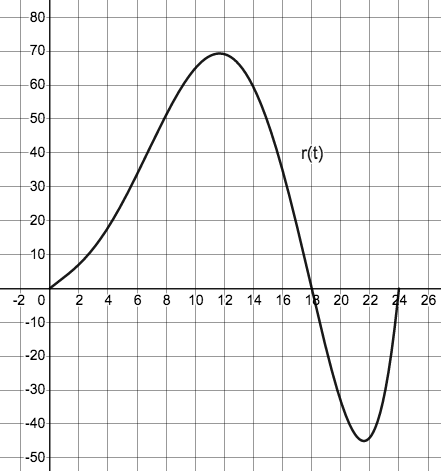
\includegraphics [scale=0.4]{I1_rate}


\begin{enumerate}
\item Over the 24 hour period, when does the tank contain the most fluid? Explain.
\vfill
\item Describe in a sentence: what does $\displaystyle \int_4^8 r(t)\,dt$ represent in this context? What do the 4 and 8 represent? What are the units? 
\vfill
\item Estimate $\displaystyle \int_0^{24} r(t)\,dt$ using 6 left-rectangles. Show your work and explain whether you think this is an over or under estimate.
\end{enumerate}

\end{document}


